\section{Projektführung}
\subsection{Rahmenplan}
\begin{figure}[H]
	\centering
	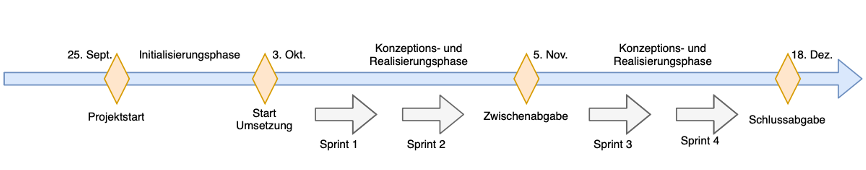
\includegraphics[width=\linewidth]{2_Projektfuehrung/Bilder/rahmenplan.png}
	\caption{Rahmenplan}
	\label{fig: Rahmenplan}
\end{figure}
Folgende Meilensteine sind gemäss Zeitstrahl zu erreichen.
\begin{center}
	\begin{tabularx}{\textwidth}{|X|X|}
		\hline
		\textbf{Meilenstein} & \textbf{Deliverable} \\
		\hline
		\textbf{Projektstart} & Beginn des Projekts, Projektteam definiert. \\
		\hline
		\textbf{Zwischenabgabe} & Rahmenplan, Projektorganisation und erste Projektrisikoliste definiert. Produktbacklog zu 80\% definiert. Sprintplanung für Sprint 1 detailliert und für Sprint 2 grob dokumentiert. \\
		\hline
		\textbf{Schlussabgabe} & Sprint 4 abgeschlossen. Nachgeführte Softwarespezifikation liegt vor und ist reviewed. Alle Komponenten sind lauffähig und demonstrierbar. Interoperabilität der Logger-Komponente ist entwickelt und demonstrierbar.. \\
		\hline
	\end{tabularx}
\end{center}
\subsection{Projektkontrolle}
\textcolor{red}{needs to be done, link zum burndownchart}
\subsection{Risikomanagement}
\subsection{Definition of Done}
